\documentclass[aspectratio=169]{beamer}
\geometry{paperwidth=160mm,paperheight=100mm}
\usepackage{beamerthemesidebar}
\usepackage{hyperref}
\usepackage{color}
\usepackage{multimedia}
\usepackage{colortbl}
\usepackage{amsmath}
\usepackage{empheq}
\usepackage{cancel}
\usepackage{amssymb}
\usepackage{amsfonts}
\usepackage{lipsum}
\usepackage{tcolorbox}
\usepackage{tabularx}
\usepackage{caption}
\usepackage{bm}

\setbeamersize{sidebar width right=0pt}
\setbeamertemplate{footline}[frame number]
%
\definecolor{orange}{RGB}{250,167,12}
\definecolor{yellow}{RGB}{246,250,12}
\definecolor{green}{RGB}{128,238,1}
\definecolor{black}{RGB}{0,0,0}
\definecolor{blue}{RGB}{0,0,255}
\definecolor{red}{RGB}{255,0,0}
\definecolor{sepia}{RGB}{94,38,18}
\newcommand{\ve}[1]{{\rm\bf {#1}}}
\newcommand{\q}[1]{\textcolor{blue}{#1}}
\newcommand{\blue}[1]{\textcolor{blue}{#1}}
\newcommand{\sepia}[1]{\textcolor{sepia}{#1}}
\newcommand{\red}[1]{\textcolor{red}{#1}}
\newcommand{\green}[1]{\textcolor{green}{#1}}
\newcommand{\yellow}[1]{\textcolor{yellow}{#1}}
\newcommand{\orange}[1]{\textcolor{orange}{#1}}
\definecolor{burlywood}{RGB}{255,211,155}
\definecolor{chocolate}{RGB}{255,127,36}
\definecolor{tan}{RGB}{210,180,140}
%
\def\onethird{{\textstyle{1\over3}}}
\def\twothirds{{\textstyle{2\over3}}}
\def\fourthirds{{\textstyle{4\over3}}}
\def\onehalf{{\textstyle{1\over2}}}
\def\threehalfs{{\textstyle{3\over2}}}
%
\newcommand{\pd}{\partial}
\newcommand{\aMLT}{\alpha_{\rm MLT}}
\newcommand{\Fconv}{F_{\rm conv}}
\newcommand{\Frad}{F_{\rm rad}}
\newcommand{\Ftot}{F_{\rm tot}}
\newcommand{\Hp}{H_p}
\newcommand{\prad}{p_{\rm rad}}
\newcommand{\pgas}{p_{\rm gas}}
\newcommand{\TTc}{T_{\rm c}}
\newcommand{\rhoc}{\rho_{\rm c}}
\newcommand{\Teff}{T_{\rm eff}}
\newcommand{\Fstar}{F_\star}
\newcommand{\pstar}{p_\star}
\newcommand{\Pstar}{P_\star}
\newcommand{\Rstar}{R_\star}
\newcommand{\rhostar}{\rho_\star}
\newcommand{\Tstar}{T_\star}
%
\title{Theoretical Astrophysics I: Physics of Sun and Stars\\
Lecture 8: Detailed Models of Stellar Evolution}
\author{\texorpdfstring{\sepia{Petri K\"{a}pyl\"{a} Ivan Mili\'{c}}\newline\blue{\url{pkapyla, milic@leibniz-kis.de}}}{}}
\institute{Institut f\"ur Sonnenphysik - KIS, Freiburg}
\date{\today}
%
\begin{document}
\frame{\titlepage}


\section{Evolution of stars - detailed picture}
%
\frame{
\frametitle{Detailed picture of stellar evolution}
\begin{itemize}
\item As opposed to the simple treatment we have adopted so far, a
  general treatment of stellar evolution needs to take into account
  the details of opacity, nuclear energy production, and equation of
  state.
\item Then the equations of stellar evolution need to be solved
  \emph{numerically} and due to their non-linearity results that might
  not be intuitively clear can arise.
\item Numerical solutions have been available since the 1950s but we
  will not go to the details here.
\item The goal of the modelling efforts is to explain the observed
  Herzsprung-Russell diagram, characterised by ($\log \Teff,\log L$)
  plane, as opposed to ($\log \rhoc, \log \TTc$) on the previous
  lecture.
\end{itemize}
}
%
%
\frame{
\frametitle{Recap: Herzsprung-Russell diagram}
\begin{minipage}{0.59\linewidth}
\begin{itemize}
\item We saw earlier that there is an observed relation between the
  luminosity and effective temperature of main sequence stars
  \begin{equation}
    \log L = \alpha \log \Teff + {\rm const.},\label{equ:logL}
  \end{equation}
  where the slope $\alpha$ is varies with $L$.
\item Another correlation exists between luminosity and mass:
  \begin{equation}
    L \propto M^\nu,\label{equ:Lmass}
  \end{equation}
  with $\nu \approx 3\ldots 5$.
\item The models need to further explain why stars cluster (i.e.,
  spend much of their lifetime) at certain regions in the diagram.
\end{itemize}
\end{minipage}
\begin{minipage}{0.4\linewidth}
\begin{figure}
%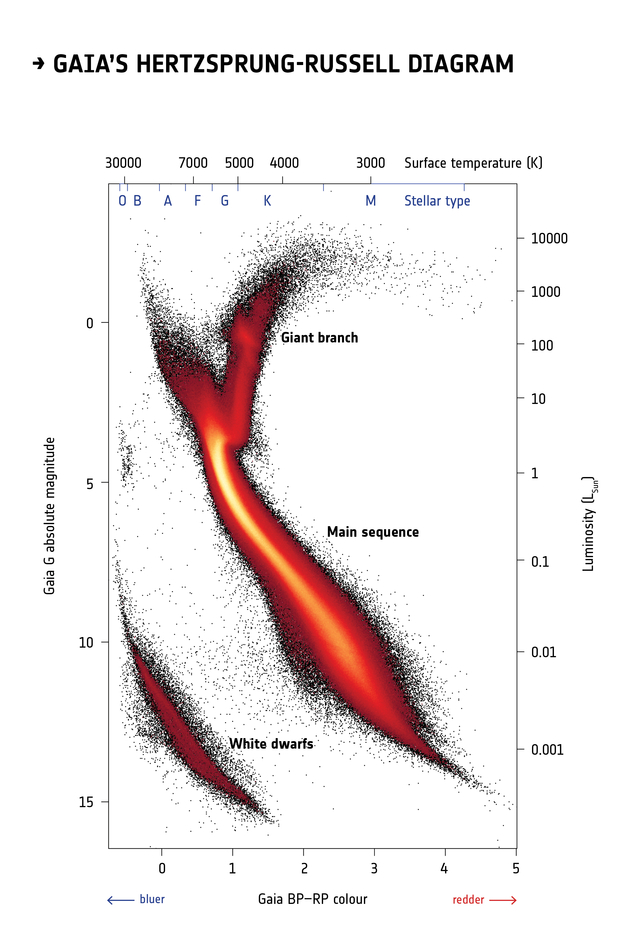
\includegraphics[width=5cm]{figures/Gaia_HR.jpg}
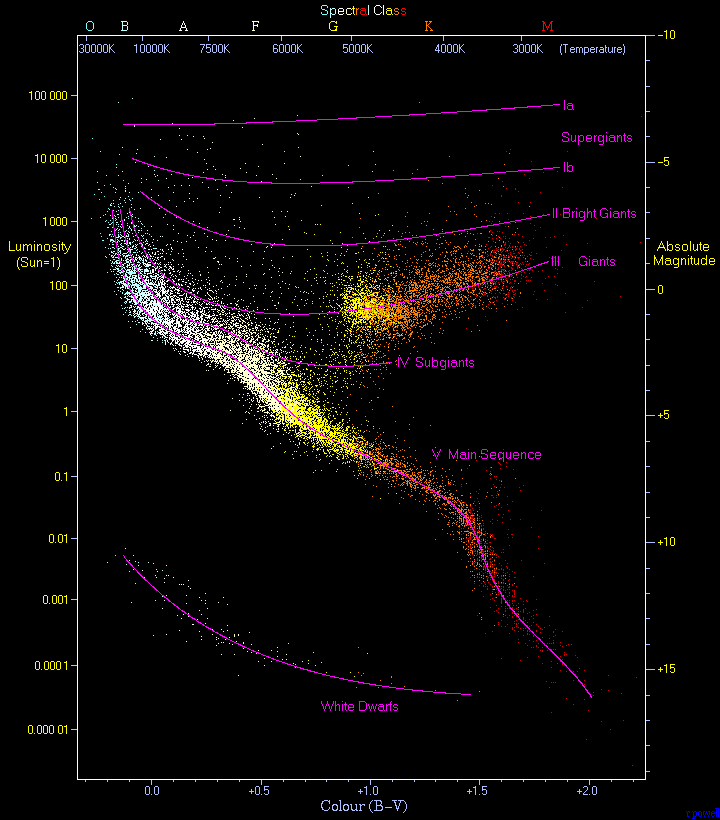
\includegraphics[width=5cm]{figures/HRDiagram.png}
\caption*{Credits: Richard Powell / Wikipedia}
\end{figure}
\end{minipage}
}
%
%
\frame{
\frametitle{Hayashi zone and pre-main-sequence phase}
\begin{itemize}
\item Assume a fully convective star of mass $M$ and radius $R$. Then
  we can adopt an interior structure corresponding to a polytrope of index $n = 1/(\gamma_{\rm a} -1)$,
  \begin{equation}
    p = K \rho^{1+\frac{1}{n}}.\label{equ:ppoly}
  \end{equation}
\item $K$ is related to $M$ and $R$ via the Lane-Emden equation:
  \begin{equation}
    K^n = C_n G^n M^{n-1} R^{3-n},\label{equ:Kn}
  \end{equation}
  where $C_n$ depends on the polytropic index $n$:
  \begin{equation}
    C_n = \frac{4\pi}{(n+1)^n} \frac{R_n^{n-3}}{M_n^{n-1}}.\label{equ:Cn}
  \end{equation}
\item $R$ is a free parameter that is fixed by joining the fully
  convective interior to a radiative photosphere above $r = R$.
\end{itemize}
}
%
%
\frame{
\frametitle{Hayashi zone and pre-main-sequence phase}
\begin{itemize}
\item The photosphere needs to be able to radiate away all of the
  incoming energy flux. This is determined by the thermodynamic
  structure, i.e., the drop of $p$, $\rho$, and $T$ accross it.
\item In Hydrostatic equilibrium
  \begin{equation}
    \frac{dp}{dr} \approx -\rho \frac{GM}{R^2},
  \end{equation}
  which can be integrated from $R$ to the point where $p$ vanishes
  \begin{equation}
    p_R = \frac{GM}{R^2}\int_R^\infty \rho dr.\label{equ:pR1}
  \end{equation}
\item Furthermore, the optical depth of the photosphere, characterised
  by $\Teff$, is of the order on unity and thus $\int_R^\infty \kappa
  \rho dr = \overline{\kappa} \int_R^\infty \rho dr$, where
  $\overline{\kappa}$ is the mean opacity in the photosphere.
\item Taking $\overline{\kappa} = \kappa(R)$ and assuming it to be a
  power law in $\rho_R$ and $\Teff$ gives:
  \begin{equation}
    \kappa_0 \rho_R^a \Teff^b \int_R^\infty \rho dr = 1.\label{equ:optau}
  \end{equation}
\end{itemize}
}
%
%
\frame{
\frametitle{Hayashi zone and pre-main-sequence phase}
\begin{itemize}
\item Combining Eqs.~(\ref{equ:pR1}) and (\ref{equ:optau}) gives:
  \begin{equation}
    p_R = \frac{GM}{R^2 \kappa_0} \rho_R^{-a} \Teff^{-b}.\label{equ:pR2}
  \end{equation}
\item Yet another relation between the thermodynamic quantities at $R$
  is given by the equation of state, here taken to be ideal gas equation:
  \begin{equation}
    p_R = \frac{\cal R}{\mu} \rho_R \Teff.\label{equ:peos}
  \end{equation}
\item Finally, the temperature at $R$ is related to the luminosity via
  \begin{equation}
    L = 4\pi R^2 \Teff^4.\label{equ:Lumi}
  \end{equation}
\item Now we have four equations that describe the surface of the
  star: Eqs.(\ref{equ:ppoly}) (with Eqs.~(\ref{equ:Kn}) and
  (\ref{equ:Cn})), (\ref{equ:pR2}), (\ref{equ:peos}), and
  (\ref{equ:Lumi})
\end{itemize}
}
%
%
\frame{
\frametitle{Hayashi zone and pre-main-sequence phase}
\begin{itemize}
\item These read in logarithmic form:
  \begin{eqnarray}
    & n \log p_R = (n-1) \log M + (3-n)\log R + (n+1) \log \rho_r + \mbox{const.} & \\
    & \log p_R = \log M - 2 \log R - a \log \rho_r - b \log \Teff + \mbox{const.} & \\
    & \log p_R = \log \rho_R + \log \Teff + \mbox{const.} & \\
    & \log L = 2 \log R + 4 \log \Teff + \mbox{const.} &
  \end{eqnarray}
\item Eliminating $\log R$, $\log \rho_R$, and $\log p_R$ yields:
  \begin{eqnarray}
    & \log L = A \log \Teff + B \log M + \mbox{const.} & \\
    & A =  \frac{(7-n)(a+1)-4-a+b}{0.5(3-n)(a+1)-1}, \ \ B = -\frac{(n-1)(a+1)+1}{0.5(3-n)(a+1)-1}. &
  \end{eqnarray}
\item This relation traces the \emph{Hayashi track} in the HR
  diagram. These should not be interpreted as evolutionary tracks but
  rather as an asymptote.
\end{itemize}
}
%
%
\frame{
\frametitle{Hayashi zone and pre-main-sequence phase}
\begin{itemize}
\item We assume for simplicity that $a = 1$ which is reasonably
  accurate, such that
  \begin{eqnarray}
    & A =  \frac{9-2n+b}{2-n}, \ \ B = -\frac{2n-1}{2-n}. &
  \end{eqnarray}
  $b$ varies much more but is usually positive
\item Dynamical stability requires that $n<3$ and therefore the
  polytropic index is limited to the range $1.5 \leq n < 3$.
\item For $b\approx 4$ and $n=1.5$ we find that $A=20$. This means
  that the Hayashi track is almost vertical in the ($\log \Teff, \log
  L$) plane.
\item As a function of mass the tracks are stacked near each other and
  higher mass leads to a shift toward higher temperatures because $A$
  and $B$ have opposite signs.
\item The slope changes with composition that can be associated with
  an effective polytropic index.
\end{itemize}
}
%
%
\frame{
\frametitle{Hayashi zone and pre-main-sequence phase}
\begin{itemize}
\item The signifigance of the Hayashi track can be seen from
  considering $\overline{\gamma}$ which is an average value of $\gamma
  = \frac{d\ln p}{d\ln\rho}$ over the whole
  star. $\overline{\gamma}_{\rm a}$ is the corresponding adiabatic
  index.
\item For a fully convective star $\overline{\gamma} =
  \overline{\gamma}_{\rm a}$.
\item If any part of the star is radiative with $\gamma<\gamma_{\rm
  a}$, then $\overline{\gamma} < \overline{\gamma}_{\rm
  a}$. Correspondingly, the average polytropic index $n>n_{\rm a}$
  where $n_{\rm a}$ is the adiabatic polytropic index defining the
  Hayashi track.
\item If $\overline{\gamma} > \overline{\gamma}_{\rm a}$, the
  situation is unstable and therefore such state is ``forbidden''. In
  practise in such a situation, convection in the star would very
  quickly restore near-adiabaticity by transporting any excess heat to
  the surface because a very small superadiabaticity is enough to
  transport massive amounts of energy (homework!).
\end{itemize}
}
%
%
\frame{
\frametitle{Hayashi zone and pre-main-sequence phase}
\begin{minipage}{0.59\linewidth}
\begin{itemize}
\item Stars from from contrating gas clouds (molecular clouds) through
  dynamical collapse. These clouds are (parsecs) and fragment in the
  process.
\item Most of the gas in such clouds is in the form of molecular
  hydrogen (H$_2$). The collapse happens in dynamical timescale
  $\tau_{\rm dyn} \propto \rho^{-1.2}$.
\item Gradually the H$_2$ molecules are dissociated, after which
  hydrogen and later helium start to be ionised. These processes use
  up most of the energy from continuing collapse and the temperature
  stays nearly constant.
\item Finally the ionisation is nearly complete and the temperature
  starts to increase and a hydrostatic equilibrium is restored. The
  object is now a protostar.
\end{itemize}
\end{minipage}
\begin{minipage}{0.4\linewidth}
\begin{figure}
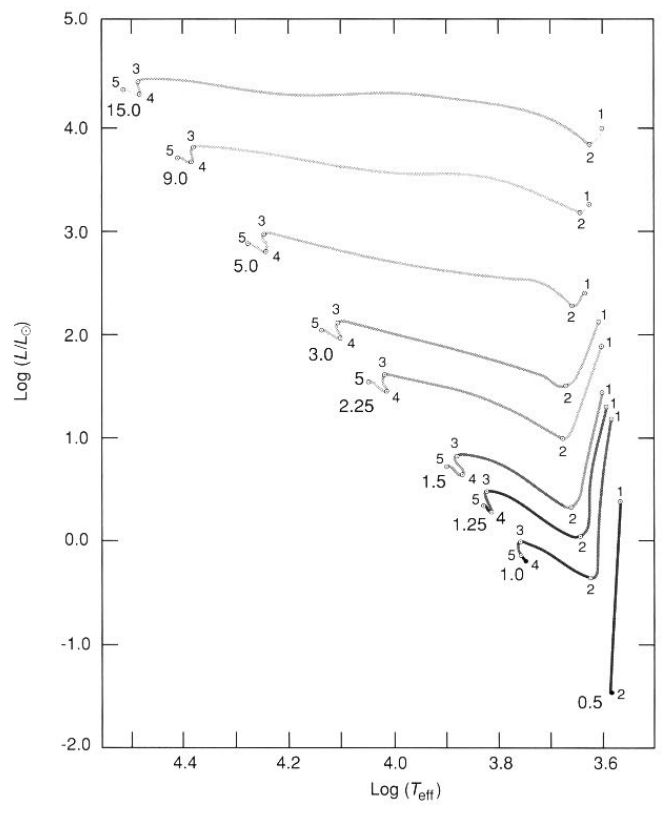
\includegraphics[width=5cm]{figures/Iben_1965_PMS.png}
\caption*{Credits: Iben (1965), Astrophys. J., 141}
\end{figure}
\end{minipage}
}
%
%
\frame{
\frametitle{Hayashi zone and pre-main-sequence phase}
\begin{minipage}{0.59\linewidth}
\begin{itemize}
\item Estimate of protostellar radius can be obtained by assuming that
  all of the gravitational energy is spent to dissociate H$_2$ and
  ionize H and He. Then,
  \begin{equation}
    \alpha \frac{GM^2}{R_{\rm ps}} \approx \frac{M}{m_{\rm H}}\left( \frac{X}{2}\chi_{{\rm H}_2} + X_{\chi_{\rm H}} + \frac{Y}{4}\chi_{\rm He} \right),
  \end{equation}
  where $\chi_{{\rm H}_2} =4.5$~eV, $\chi_{\rm H} = 13.6$~eV, and
  $\chi_{\rm He} = 79$~eV.
\item Taking $Y \approx 1 -X$ and $\alpha = \onehalf$ gives
  \begin{equation}
    \frac{R_{\rm ps}}{R_\odot} \approx \frac{50}{1-0.2X} \frac{M}{M_\odot}.
  \end{equation}
\end{itemize}
\end{minipage}
\begin{minipage}{0.4\linewidth}
\begin{figure}
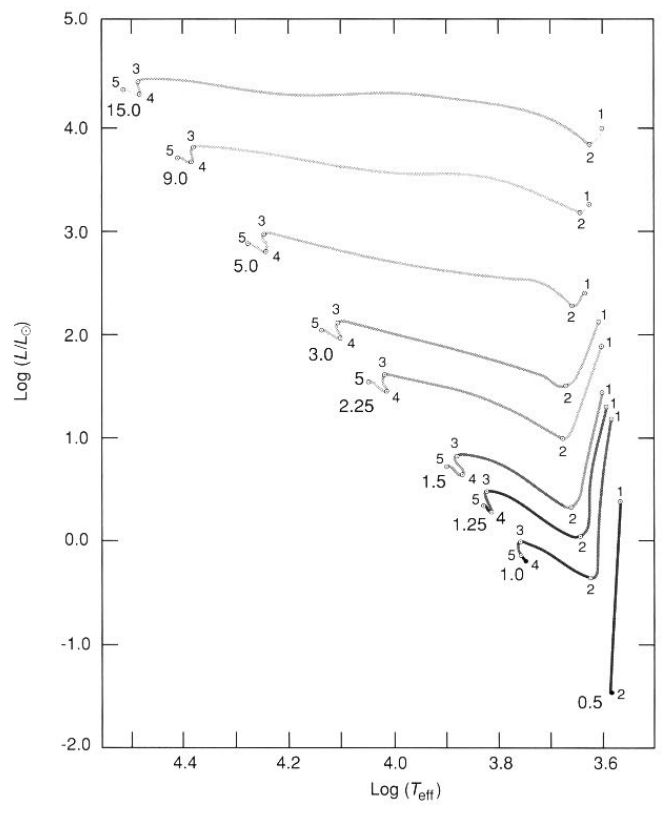
\includegraphics[width=5cm]{figures/Iben_1965_PMS.png}
\caption*{Credits: Iben (1965), Astrophys. J., 141}
\end{figure}
\end{minipage}
}
%
%
\frame{
\frametitle{Hayashi zone and pre-main-sequence phase}
\begin{minipage}{0.59\linewidth}
\begin{itemize}
\item Recalling the average temperature from virial theorem and
  inserting the estimate for $R_{\rm ps}$ with $X=0.7$ gives:
  \begin{equation}
    \overline{T} = \frac{\alpha}{3} \frac{\mu}{k} \frac{GMm_{\rm H}}{R_{\rm ps}} \approx 6\cdot 10^4~{\rm K}.
  \end{equation}
  Note that the temperature is independent of $M$.
\item At this starting point on the Hayashi track the star is fully
  convective and the gas is still opaque.
\item Contraction continues until all of the gas is ionized. The
  opacity drops first in the interior and the convection zone recedes.
  $\Teff$ starts to rise slowly.
\item Nuclear reactions start gradually when core temperature
  increases and increase the luminosity. Evolutionary track is
  complicated by ignition of different branches of hydrogen burning.
\end{itemize}
\end{minipage}
\begin{minipage}{0.4\linewidth}
\begin{figure}
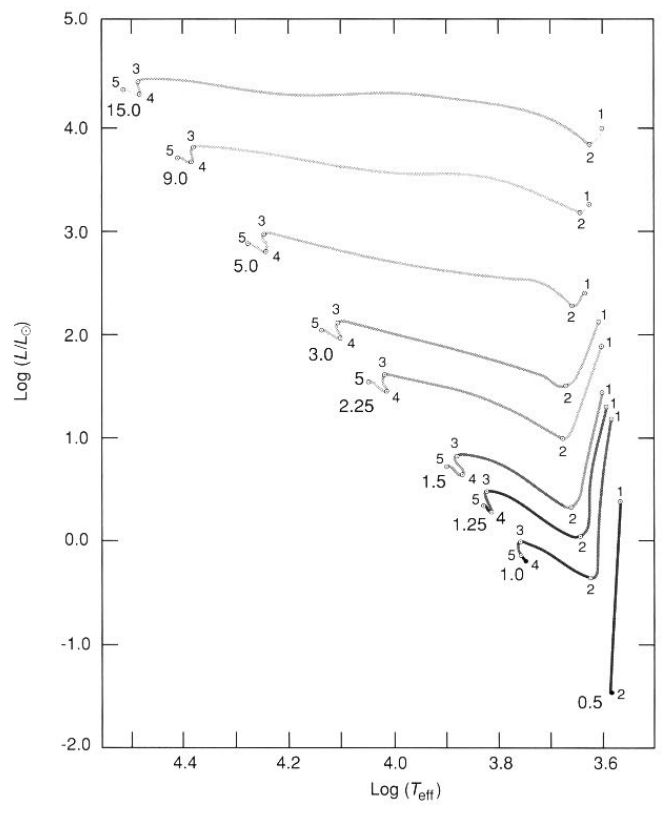
\includegraphics[width=5cm]{figures/Iben_1965_PMS.png}
\caption*{Credits: Iben (1965), Astrophys. J., 141}
\end{figure}
\end{minipage}
}
%
%
\frame{
\frametitle{Hayashi zone and pre-main-sequence phase}
\begin{minipage}{0.59\linewidth}
\begin{figure}
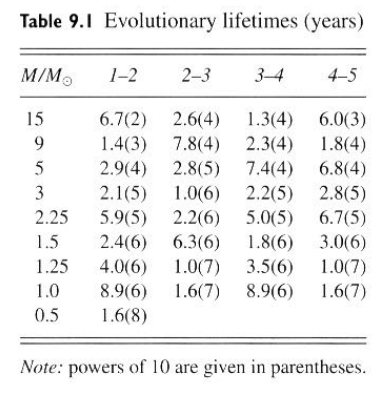
\includegraphics[width=5cm]{figures/Prialnik_PMS_lifetimes.png}
\caption*{Credits: Prialnik.}
\end{figure}
\begin{itemize}
\item The time that stars spend in the PMS phase depends strongly on
  the mass.
\end{itemize}
\end{minipage}
\begin{minipage}{0.4\linewidth}
\begin{figure}
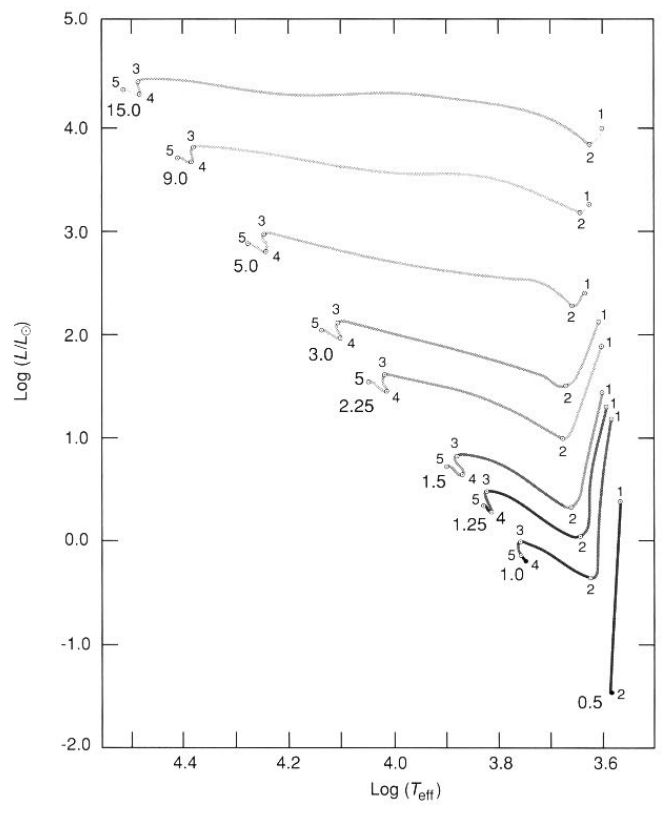
\includegraphics[width=5cm]{figures/Iben_1965_PMS.png}
\caption*{Credits: Iben (1965), Astrophys. J., 141}
\end{figure}
\end{minipage}
}
%
\frame{
\frametitle{Main-sequence phase}
\begin{itemize}
\item TBA
\end{itemize}
}
%
%
\frame{
\frametitle{Main-sequence phase}
\begin{itemize}
\item TBA
\end{itemize}
}
%
%
\frame{
\frametitle{Main-sequence phase}
\begin{itemize}
\item TBA
\end{itemize}
}
%
%
\frame{
\frametitle{Red Giant phase}
\begin{itemize}
\item TBA
\end{itemize}
}
%
%
\frame{
\frametitle{Red Giant phase}
\begin{itemize}
\item TBA
\end{itemize}
}
%
%
\frame{
\frametitle{Red Giant phase}
\begin{itemize}
\item TBA
\end{itemize}
}
%
%
%
\end{document}
% 

